\documentclass[12pt]{article}
\usepackage{graphicx}
\usepackage[none]{hyphenat}
\usepackage{graphicx}
\usepackage{listings}
\usepackage[english]{babel}
\usepackage{graphicx}
\usepackage{caption} 
\usepackage{booktabs}
\usepackage{array}
\usepackage{amssymb} % for \because
\usepackage{amsmath}   % for having text in math mode
\usepackage{extarrows} % for Row operations arrows
\usepackage{listings}
\lstset{
  frame=single,
  breaklines=true
}
\usepackage{hyperref}
  
%Following 2 lines were added to remove the blank page at the beginning
\usepackage{atbegshi}% http://ctan.org/pkg/atbegshi
\AtBeginDocument{\AtBeginShipoutNext{\AtBeginShipoutDiscard}}


%New macro definitions
\newcommand{\mydet}[1]{\ensuremath{\begin{vmatrix}#1\end{vmatrix}}}
\providecommand{\brak}[1]{\ensuremath{\left(#1\right)}}
\providecommand{\norm}[1]{\left\lVert#1\right\rVert}
\providecommand{\abs}[1]{\left\vert#1\right\vert}
\newcommand{\solution}{\noindent \textbf{Solution: }}
\newcommand{\myvec}[1]{\ensuremath{\begin{pmatrix}#1\end{pmatrix}}}
\let\vec\mathbf


\begin{document}

\begin{center}
\title{\textbf{Conic Sections - Ellipse}}
\date{\vspace{-5ex}} %Not to print date automatically
\maketitle
\end{center}
\setcounter{page}{1}

\section{11$^{th}$ Maths - Chapter 11}
This is Problem-3 from Exercise 11.3
\begin{enumerate}
\item Find the coordinates of the focii, the vertices, the length of major and minor axes, the eccentricity and the length of the latus rectum of an ellipse whose equation is given by $\frac{x^2}{16}+\frac{y^2}{9}=1$.

\solution
The given equation of ellipse can be rearranged as 
\begin{align}
 9x^2+16y^2-144=0\label{eq:eq1}
\end{align}
The above equation can be equated to the general equation of conic sections
\begin{align}
 g\brak{\vec{x}}=\vec{x}^\top \vec{V} \vec{x} + 2\vec{u}^\top \vec{x} + f = 0\label{eq:eq2}
\end{align}
From \eqref{eq:eq1} and \eqref{eq:eq2}
\begin{align}
 \vec{V} &= \myvec{9&0\\0&16}\label{eq:eq3}\\
 \vec{u} &= \vec{0}\\
 f &= -144
\end{align}
From \eqref{eq:eq3} the eigen values $\lambda_1 \text{ and } \lambda_2$ are given as
\begin{align}
 \lambda_1 &= 9\\
 \lambda_2 &= 16
\end{align}
\begin{enumerate}
\item The eccentricity of the ellipse is given as
\begin{align}
 e &= \sqrt{1 - \frac{\lambda_1}{\lambda_2}} \\
          &= \sqrt{1-\frac{9}{16}}\\
   &= \frac{\sqrt{7}}{4}
\end{align}
\item Finding the coordinates of Focii
\begin{align}
 \vec{F} &= \pm e\sqrt{\frac{\abs{f_0}}{\lambda_2\brak{1-e^2}}}\Vec{e_1}\\
\text{Where }f_0 &=-f\\
 \vec{F} &= \pm\sqrt{7}\myvec{1\\0}\\
	&= \pm\myvec{\sqrt{7}\\0}
\end{align}
\item The length of the major axis is given by
\begin{align}
 &2\sqrt{\abs{\frac{f_0}{\lambda_1}}}\\
        &2\sqrt{\abs{\frac{144}{9}}}= 8
\end{align}
\item The length of minor axis is given by
\begin{align}
 &2\sqrt{\abs{\frac{f_0}{\lambda_2}}}\\
        &2\sqrt{\abs{\frac{144}{16}}}= 6
\end{align}
\item The vertices of the ellipse are given by
\begin{align}
 \pm \myvec{0\\\sqrt{\abs{\frac{f_0}{\lambda_2}}}}= \pm \myvec{0\\4}
\end{align}
\item The length of latus rectum is given as
\begin{align}
 &2\frac{\sqrt{\abs{f_0 \lambda_1}}}{\lambda_2} \\
 &= 2\frac{\sqrt{\abs{144\brak{9}}}}{16}\\
 &= \frac{9}{2}
\end{align}
\begin{figure}[!h]
	\begin{center}
		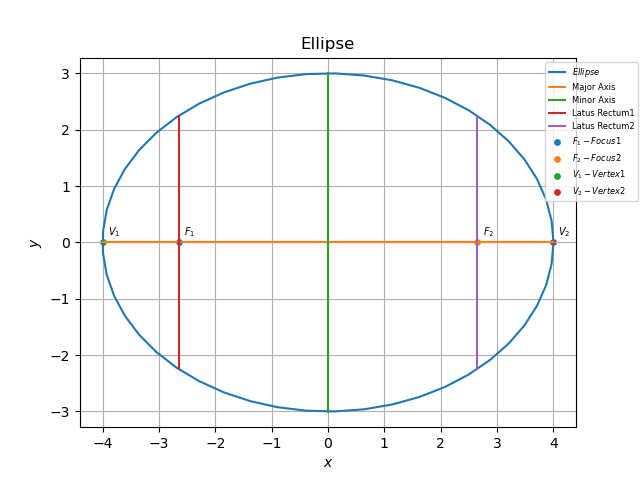
\includegraphics[width=\columnwidth]{figs/conic.png}
	\end{center}
\caption{}
\label{fig:Fig1}
\end{figure}
\end{enumerate}
\end{enumerate}
\end{document}
